%%
%    * ----------------------------------------------------------------
%    * "THE BEER-WARE LICENSE" (Revision 42/023):
%    * Ronny Bergmann <mail@rbergmann.info> wrote this file. As long as
%    * you retain this notice you can do whatever you want with this
%    * stuff. If we meet some day and you think this stuff is worth it,
%    * you can buy me a beer or a coffee in return.
%    * ----------------------------------------------------------------
%
%
% A german example using the Kartei.cls - including print and toc as
% options, hence all pages are Din A4.
%
% Last Change: Kartei 1.9, 2012/01/04
%
\documentclass[a6paper,10pt,grid=front%
,toc
%,print
]{kartei}
\usepackage[utf8]{inputenc} %UTF8
\usepackage{hyperref}
\begin{document}
  \setcardpagelayout

  \section*{ANS08}

  \begin{karte}{Definition Data Warehouse}    
    Ein Data Warehouse dient dazu, Daten aus unterschiedlichen internen und externen Quellen zusammenzuführen und zu speichern, um anschließend mithilfe unterschiedlicher Abfrage-, Analyse- und Auswertungsprogrammen neue Informationen zu gewinnen.
  \end{karte}

  \begin{karte}{Worin besteht der Unterschied zwischen operativen \& analytischen Daten?}
    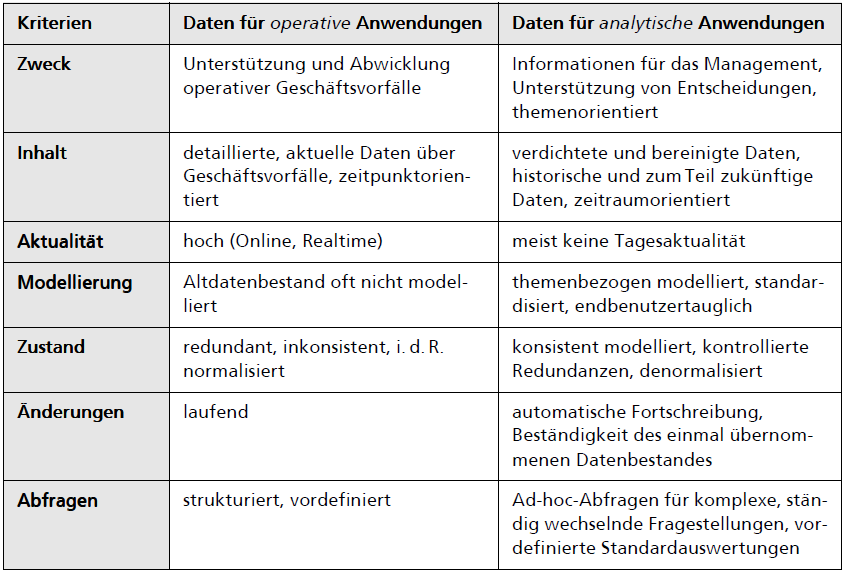
\includegraphics[width=0.9\textwidth]{img/diff_operativ_analytische_daten}
  \end{karte}

  \begin{karte}{Ziele eines Data Warehouse?}
    \begin{itemize}
      \item Informationen für das Management
      \item Unterstützung von Entscheidungen
      \item zusammenführen unterschiedlicher Daten aus operativen Anwendungssystemen
      \item es werden (un-)strukturierte Daten übernommen
      \item Veränderung, Aggregation der Daten
    \end{itemize}
  \end{karte}

  \begin{karte}{Aufbau analytischer Informationssysteme}
    \begin{itemize}
      \item \textbf{Zentrales DWH} enthält eine von den operativen Systemen isolierte Datenbank
      \item \textbf{Data Mart} ist ein subjektspezifisches oder abteilungsspezifisches DWH; entweder Datenbestände gleichzeitig an mehreren Orten schneller bereitzustellen oder einzelne Fachabteilungen spezifische Daten zu liefern
    \end{itemize}
    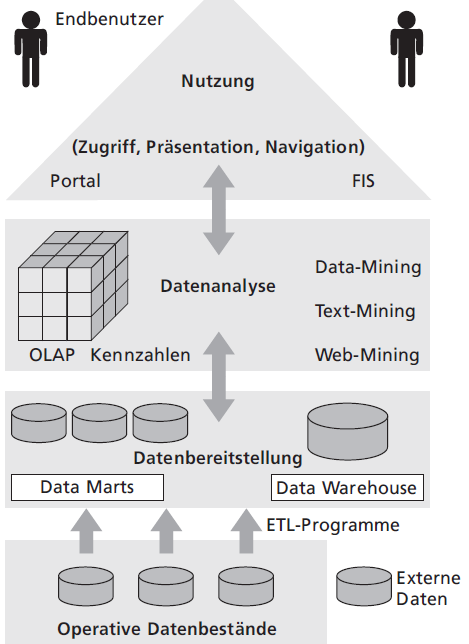
\includegraphics[height=0.5\paperheight]{img/aufbau_analytischer_is}    
  \end{karte}

  \begin{karte}{Unterschied Data Warehouse \& Data Mart}
    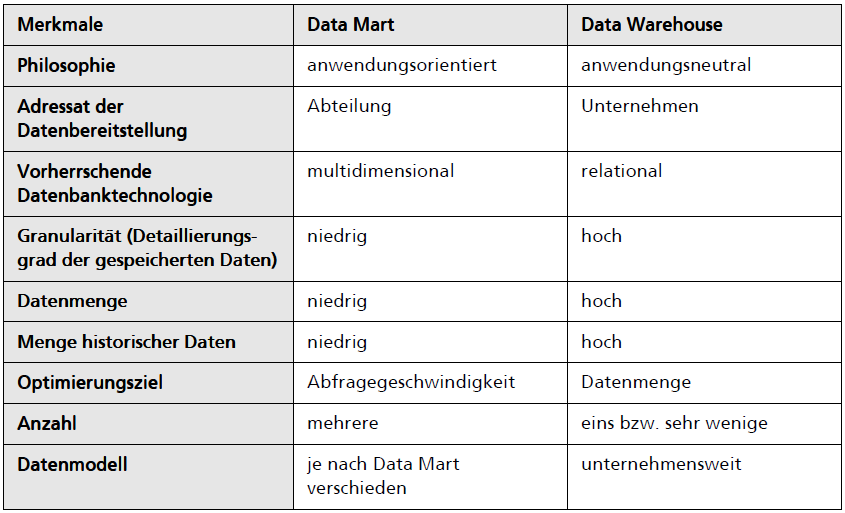
\includegraphics[width=0.9\paperheight]{img/diff_dwh_dm}
  \end{karte}

  \begin{karte}{Ablauf ETL?}
    \begin{itemize}
      \item Analyse und Dokumentation operativer und externer Datenquellen
      \item Extrahieren der ausgewählten Daten
      \item Transformation operativer Daten
      \item Bereinigung transformierter Daten
      \item periodisches Laden der Daten ins DWH
    \end{itemize}
  \end{karte}

  \begin{karte}{Extraktion}
    Unter Extraktion versteht man die Selektion der Daten aus den (zumeist) operativen Datenquellen und ihre anschließende Speicherung in einen Arbeitsbereich des DWH (Staging Area). Hier werden die Daten zwischengespeichert und transformiert bzw. bereinigt und im Anschluss in das DWH übertragen.
  \end{karte}

  \begin{karte}{Wann wird die Extraktion durchgeführt?}
      \begin{itemize} 
      \item Periodisch
      \item Anfrage
      \item Ereignisgesteuert (wenn z.B. Werte unterschritten werden)
      \item Sofort (DWH hat die gleiche Aktualität wie die operativen Systeme)
    \end{itemize}
  \end{karte}

  \begin{karte}{Transformation}
      Transformation findet in der s.g. Staging Area statt und bereinigt bzw. transformiert die Quelldaten in das gewünschte Zielformat.
  \end{karte}

  \begin{karte}{Qualitätsmängel der Quelldaten}
    \begin{itemize} 
      \item inkorrekte Daten (Eingabe-/Verarbeitungsfehler)
      \item logisch widersprüchliche Daten
      \item unvollständige, ungenaue, zu grobe Daten
      \item redundante Daten
      \item uneinheitliche Daten
      \item veraltete Daten
      \item irrelevante Daten
      \item unverständliche Daten (wegen qualitativ mangelhafter Metadaten)
    \end{itemize}

    \textbf{Verfahren:}
    \begin{itemize}
      \item Bereinigung
      \item Harmonisierung (betriebswirtschaftlich: Codierung, Schlüssel, Attribute)
      \item Verdichtung (für Analysezwecke aggregiert werden $\rightarrow$ Regionalzahlen usw.)
      \item Anreicherung (Ergänzung um errechnete Kennzahlen)
    \end{itemize}
  \end{karte}

  \begin{karte}{Bereinigung - Was ist zu beachten?}
    \begin{itemize} 
      \item Muss-Feld?
      \item Plausibilitätsprüfung bei der Eingabe?
      \item Wir das Feld gemäß der ursprünglichen Bestimmung genutzt?
      \item Wurde das Datenfeld nachträglich aufgenommen? (fehlt bei älteren Daten dann)
      \item Existieren konkrete Änderungspläne für die operativen Daten?
    \end{itemize}    
  \end{karte}

  \begin{karte}{Daten-Mängel}
    Es werden \textbf{syntaktische} und \textbf{semantische} Mängel unterschieden.

    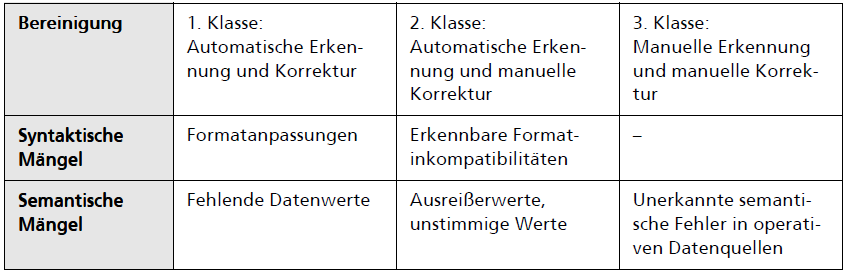
\includegraphics[width=0.9\textwidth]{img/maengel}
  \end{karte}

  \begin{karte}{Harmonisierung - Was wird getan?}
    \begin{itemize}
      \item Vereinheitlichung unterschiedlicher Codierungen (z.B. männlich, m, 1, weiblich, w, 0)
      \item Synonyme und Homonymen (unterschiedliche Attributnamen mit gleicher Bedeutung z.B. vorname, vname, firstname)
      \item Harmonisierung von Schlüsseln und Kennzahlen      
    \end{itemize}
  \end{karte}

  \begin{karte}{Verdichtung}
    Es werden Daten im DWH (Staging Area) auf verschiedenen Stufen aufsummiert.
    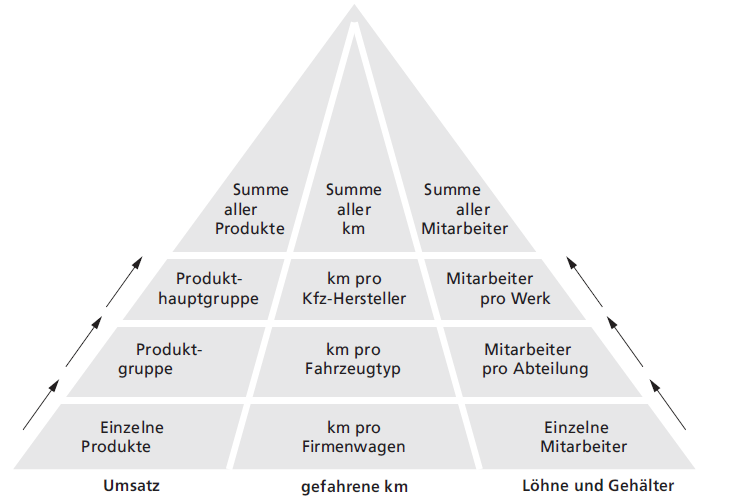
\includegraphics[width=0.9\textwidth]{img/verdichtung}
  \end{karte}

  \begin{karte}{Anreicherung}
    Es werden Berechnungen durchgeführt, die zusammen mit den übrigen analytischen Daten gespeichert werden, d.h. es werden konkrete Kennzahlen ermittelt basierend auf einem gegeben Kennzahlensystem (z.B. DuPont-Schema $\rightarrow$ ROI)

    Vorteile der Anreicherung sind:
    \begin{itemize}
      \item kürzere Antwortzeiten bei späteren Anfragen da es sich um vorberechnete Werte handelt
      \item hohe Datenkonsistenz, da sie nach einem einheitlichen Algorithmus berechnet werden
    \end{itemize}
  \end{karte}  

%  \begin{karte}{}
%
%  \end{karte}

\end{document}